\section{}

Die Abbildung $f \colon \Real \to \Real$, $x \mapsto x^3 + 3x$ ist stetig mit $\lim_{x \to -\infty} f(x) = -\infty$ und $\lim_{x \to \infty} f(x) = \infty$;
nach dem Zwischenwertsatz ist $f$ deshalb surjektiv.
Außerdem ist $f$ differenzierbar mit $f'(x) = 3 x^2 + 3 > 0$ für alle $x \in \Real$, weshalb $f$ streng monoton steigend, und somit injektiv ist.
Die Abbildung $f$ ist also bijektiv, weshalb die Gleichung $f(x) = a$ für jedes $a \in \Real$ eine eindeutige reelle Lösung besitzt.

Mithilfe von scipy lassen sich die drei verschiedenen Lösungen bestimmen:

\lstinputlisting[style=pythoncode, firstline = 1, lastline = 5]{chapter_05/exercise_05_26.py}

Wir erhalten die folgenden Lösungen:

\begin{consoleoutput}
{-(-1/2 - sqrt(3)*I/2)*(-27*a/2 + sqrt(729*a**2 + 2916)/2)**(1/3)/3 + 3/((-1/2 - sqrt(3)*I/2)*(-27*a/2 + sqrt(729*a**2 + 2916)/2)**(1/3)), -(-1/2 + sqrt(3)*I/2)*(-27*a/2 + sqrt(729*a**2 + 2916)/2)**(1/3)/3 + 3/((-1/2 + sqrt(3)*I/2)*(-27*a/2 + sqrt(729*a**2 + 2916)/2)**(1/3)), -(-27*a/2 + sqrt(729*a**2 + 2916)/2)**(1/3)/3 + 3/(-27*a/2 + sqrt(729*a**2 + 2916)/2)**(1/3)}
\end{consoleoutput}

Wir können nun die reelle Lösung im geforderten Intervall $[-500, 500]$ plotten.

\begin{center}
  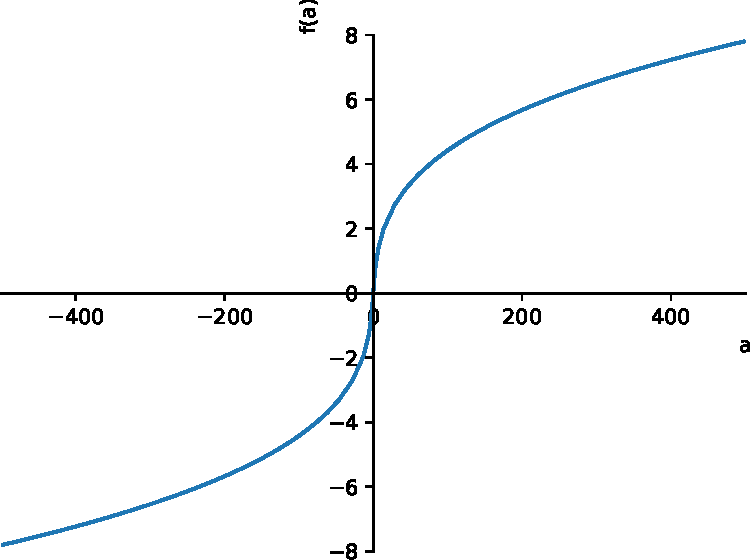
\includegraphics[width = \textwidth]{chapter_05/exercise_05_26_figure.pdf}
\end{center}

